\chapter{\textit{Python}}

\section{Sejarah \textit{Python}}
Python merupakan bahasa pemrograman tingkat tinggi yang dapat digunakan banyak hal, \textit{Python} awalnya dirancang oleh \textbf{Guido van Rossum} pada tahun 1980 yang mana nama \textit{Python} sebelum sebesar sekarang yaitu \textit{ABC Programming Language} yang dijalankan di sistem operasi bernama \textit{Amoeba Operating System}. Guido merasakan kehebatan dan kemampuan serta fitur yang berada pada bahasa pemrograman ABC ini sehingga Guido mengambil siktaks-sintaks yang berada pada bahasa pemrograman ABC ini, tentu saja banyak komplain yang berdatangan sehingga Guido terus melakukan perbaikan pada bahasa pemrograman yang sedang ia buat kala itu. Lalu, disinilah nama \textit{Python} muncul dimuka bumi sebagai bahasa pemrograman, disaat Guido sedang menonton televisi dan menemukan kata '\textit{Monty Python's Flying Circus}'.

Bahasa \textit{Python} secara resmi dirilis pada tahun 1991, saat rilis pertama kali semua orang terkejut dengan sintaks yang dimiliki oleh \textit{Python} ketika dibandingkan dengan bahasa lain seperti \textit{Java, C, C++}, dan lain-lain pengekspresian bahasa ini cukup sederhana. Tujuan dari dibuatnya bahasa pemrograman ini adalah untuk mempermudah dalam membaca sebuah kode dari penulisan sintaks dan produktivitas dalam hal pengembangan tingkat lanjut.

\section{Perbedaan \textit{Python 2.x} dan \textit{Python 3.x}}
Banyak perbedaan yang akan kita temui jika kita dahulu pernah menggunakan \textit{python} versi 2.x cukup lama sehingga berpindah ke versi 3.x, berikut contoh perbedaan pada \textit{python} versi 2.x dan 3.x yang sangat penting untuk diketahui:

\begin{enumerate}

\item Perintah \textbf{print}
Perbedaan perintah \textit{print} pada dua versi ini adalah python 2.x tidak memakai kurung dan 3.x memakai kurung untuk perintah \textit{print} bisa dilihat pada gambar ~\ref{print} dan \ref{printnano}

\begin{figure}[H]
\centering
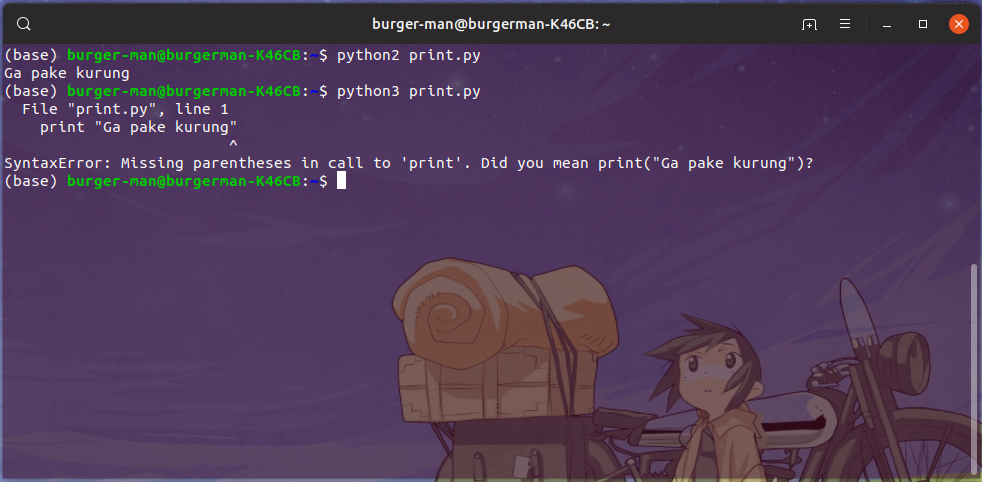
\includegraphics[width=1\textwidth]{figures/print.png}
\caption{Gambar hasil print}
\label{print}
\end{figure}

\begin{figure}[H]
\centering
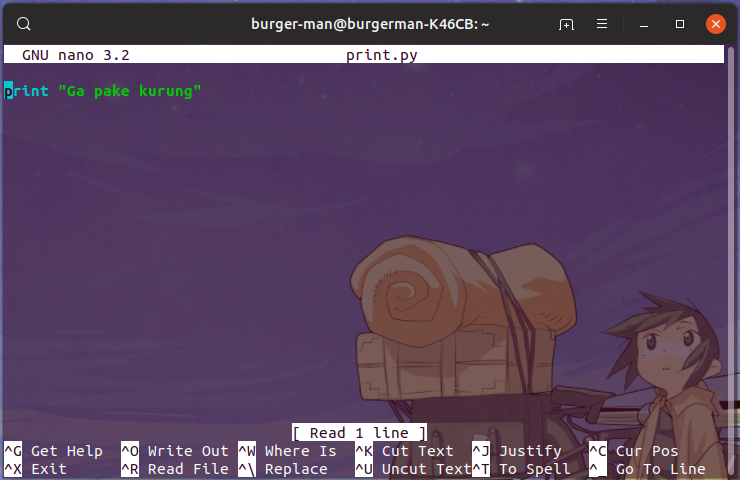
\includegraphics[width=1\textwidth]{figures/printnano.png}
\caption{Gambar perintah print}
\label{printnano}
\end{figure}

\item Perintah pembagian \textbf{\textit{integer}}
Hasil dari perintah pembagian cukup jelas berbeda yang mana versi 2.x tidak secara mendetail untuk hasilnya sehingga angka yang dihasilkan bilangan \textbf{\textit{integer}} sedangkan versi 3.x bertipe \textbf{\textit{float}} perbedaannya bisa dilihat pada gambar \ref{div} dan \ref{divnano}.

\begin{figure}[H]
\centering
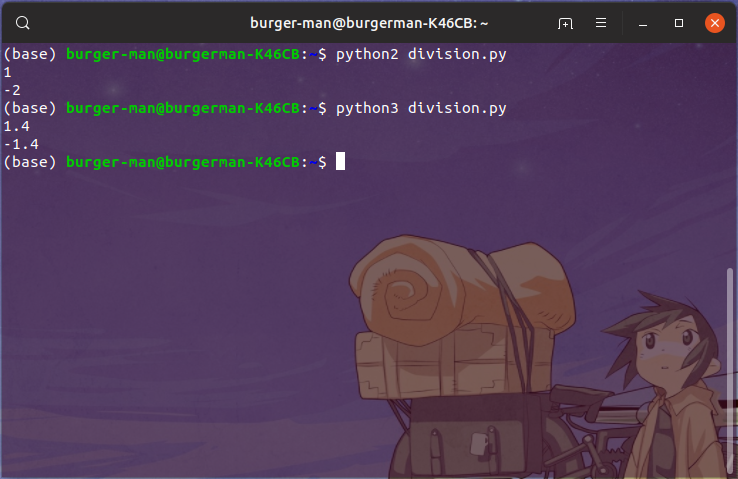
\includegraphics[width=1\textwidth]{figures/div.png}
\caption{Gambar hasil pembagian}
\label{div}
\end{figure}

\begin{figure}[H]
\centering
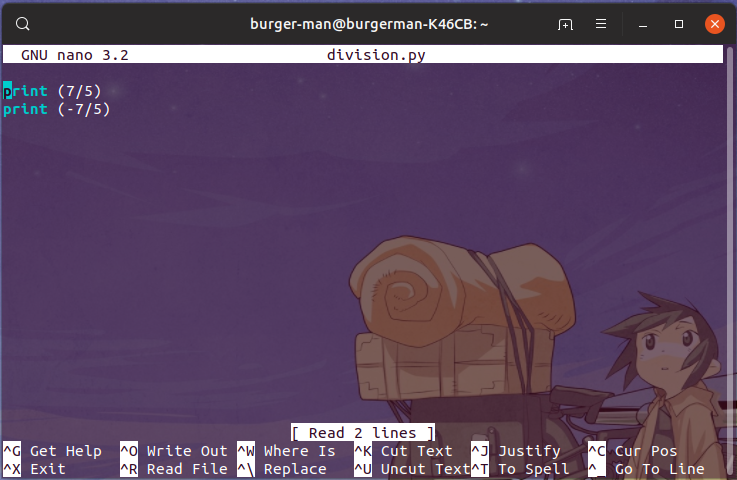
\includegraphics[width=1\textwidth]{figures/divnano.png}
\caption{Gambar perintah pembagian}
\label{divnano}
\end{figure}

\item \textit{\textbf{Try and Except}}
Perbedaan pada \textit{try and expcept} hanya berbeda di penggunaan \textbf{,} untuk versi 2.x dan \textbf{as} untuk versi 3.x.

\begin{figure}[H]
\centering
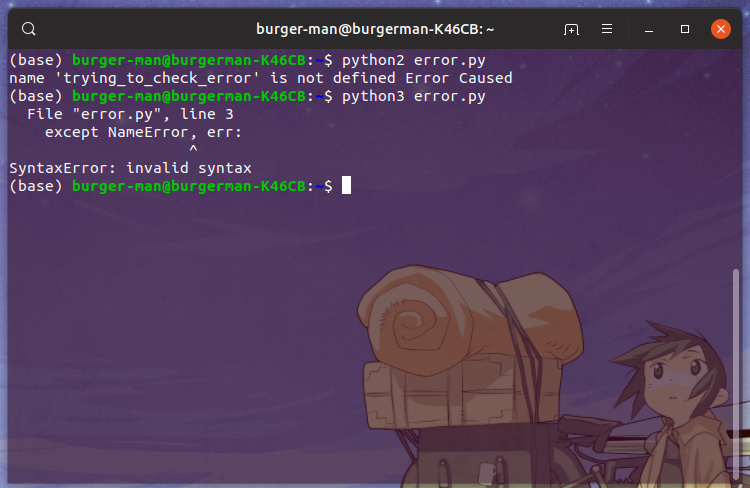
\includegraphics[width=1\textwidth]{figures/error.png}
\caption{Gambar hasil error}
\label{error}
\end{figure}

\begin{figure}[H]
\centering
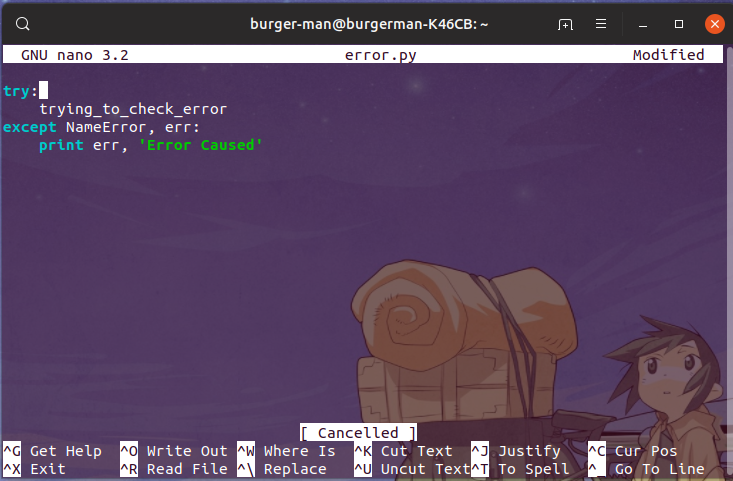
\includegraphics[width=1\textwidth]{figures/errornano.png}
\caption{Gambar perintah error}
\label{errornano}
\end{figure}

\item \textbf{\textit{Looping}}
Perbedaan pada looping hanya saja versi 3.x tidak bisa menggunakan sintaks \textbf{\textit{xrange}} lagi.

\begin{figure}[H]
\centering
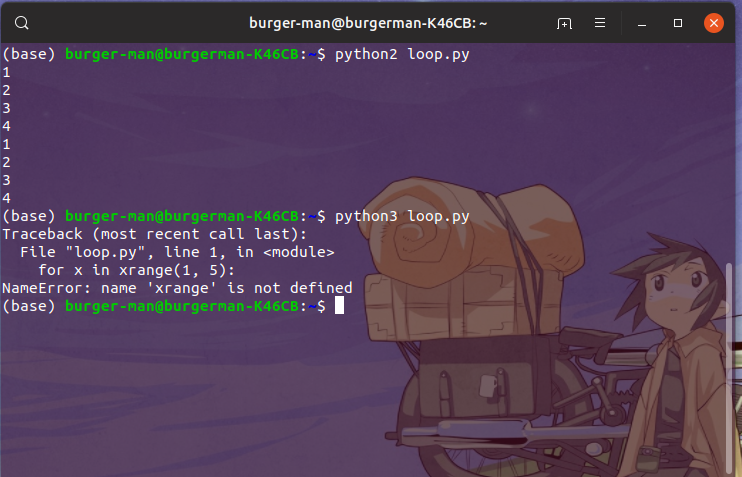
\includegraphics[width=1\textwidth]{figures/loop.png}
\caption{Gambar hasil looping}
\label{loop}
\end{figure}

\begin{figure}[H]
\centering
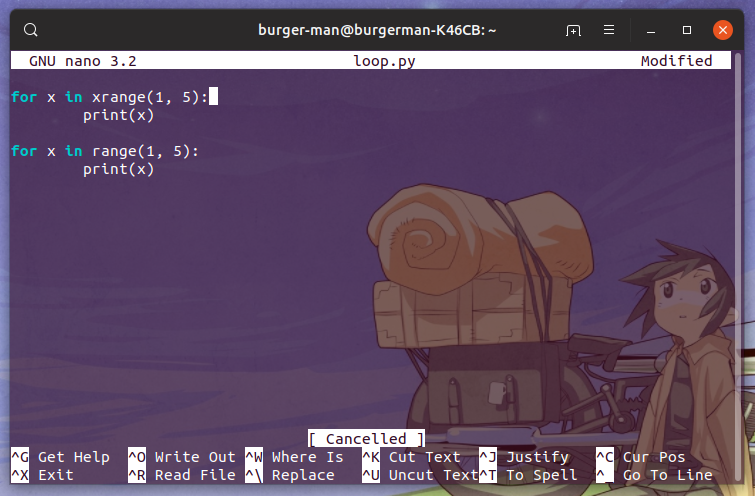
\includegraphics[width=1\textwidth]{figures/loopnano.png}
\caption{Gambar perintah looping}
\label{loopnano}
\end{figure}

\item \textbf{\textit{Unicode}}
Unicode ini cukup penting karena kita mengetahui bagaimana setiap versi merespons setiap unicode yang diberikan.

\begin{figure}[H]
\centering
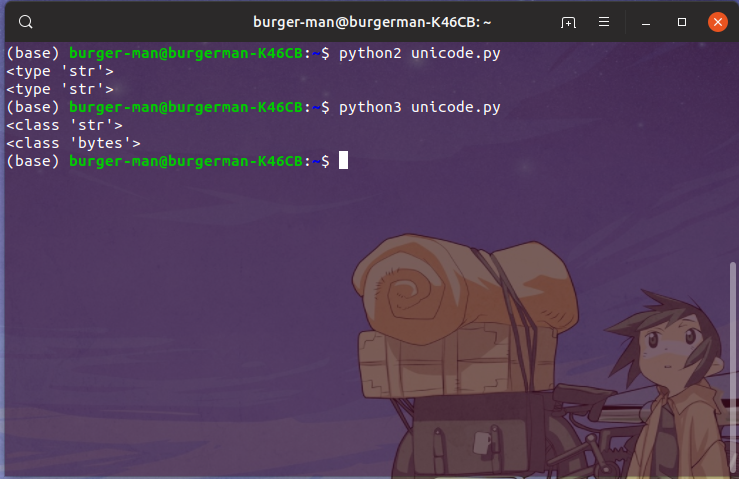
\includegraphics[width=1\textwidth]{figures/unicodebytes.png}
\caption{Gambar hasil unicode (bytes)}
\label{unibytes}
\end{figure}

\begin{figure}[H]
\centering
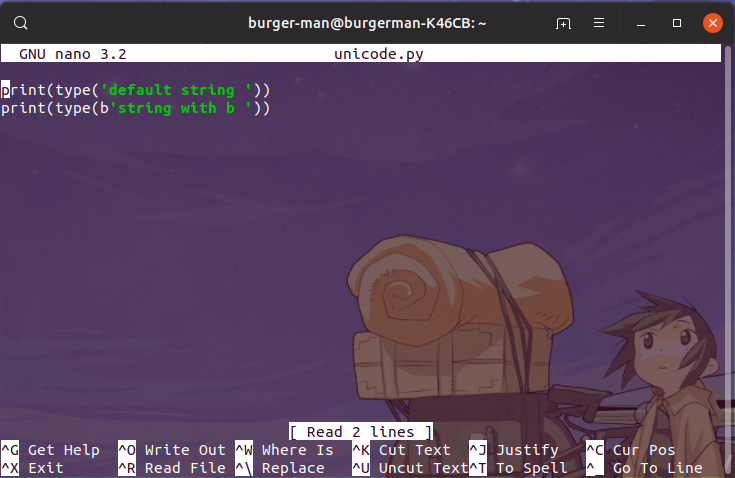
\includegraphics[width=1\textwidth]{figures/unicodebytesnano.png}
\caption{Gambar perintah unicode (bytes)}
\label{unibytesnano}
\end{figure}
Pada gambar ~\ref{unibytes} terlihat jelas bahwa perintah \textbf{\textit{bytes}} hanya direspon pada versi 3.x sedangkan versi 2.x merespon \textbf{\textit{string}}

\begin{figure}[H]
\centering
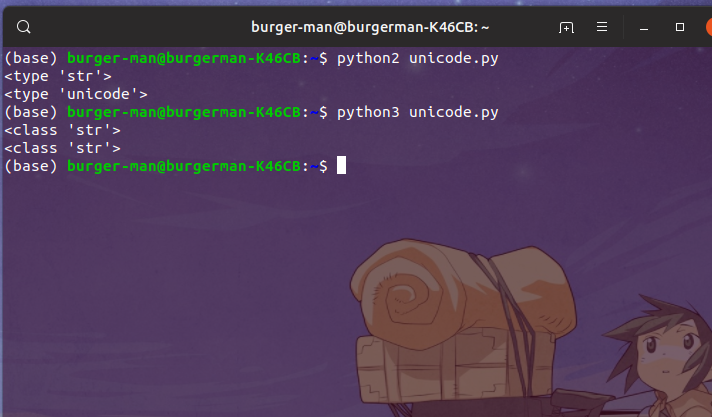
\includegraphics[width=1\textwidth]{figures/unicodeuni.png}
\caption{Gambar hasil unicode}
\label{unicodeuni}
\end{figure}

\begin{figure}[H]
\centering
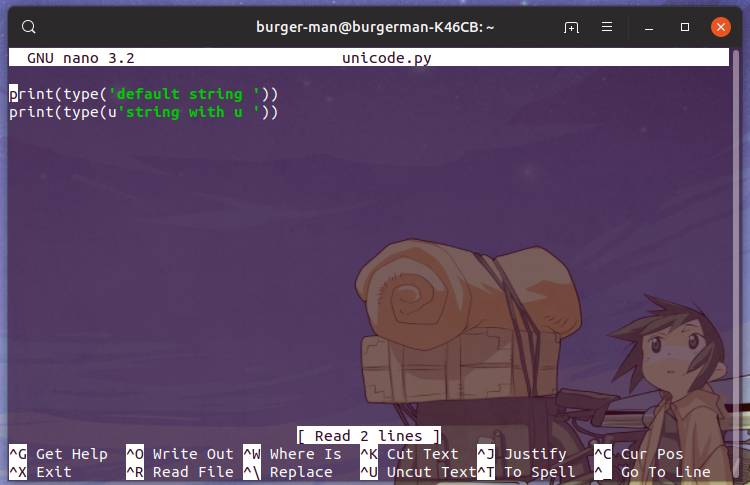
\includegraphics[width=1\textwidth]{figures/unicodeuninano.png}
\caption{Gambar perintah unicode}
\label{unicodeuninano}
\end{figure}

\end{enumerate}